
% JuliaCon proceedings template
\documentclass{juliacon}
\setcounter{page}{1}

\usepackage{amsmath}
\usepackage{amssymb}
\usepackage{bm}
\usepackage{multirow}
\usepackage{svg}
\usepackage{calc}
\usepackage{algorithm}
\usepackage{algorithmicx}
\usepackage{algpseudocode}
\usepackage{url}
\usepackage{subcaption}
\graphicspath{{figures/}}

\begin{document}

% **************GENERATED FILE, DO NOT EDIT**************

\title{Tracking.jl: Accelerating multi-antenna GNSS receivers with CUDA}

\author[1]{Can Özmaden}
\affil[1]{Faculty of Electrical Engineering and Information Technology, Chair of Navigation, RWTH Aachen University}

\keywords{Julia, GNSS, Signal Processing, SDR, CUDA, GPU}

\hypersetup{
pdftitle = {Tracking.jl: Accelerating multi-antenna GNSS receivers with CUDA},
pdfsubject = {JuliaCon 2019 Proceedings},
pdfauthor = {Can Özmaden},
pdfkeywords = {Julia, GNSS, Signal Processing, SDR, CUDA, GPU},
}



\maketitle

\begin{abstract}

    The use of advanced Global Navigation Satellite System (GNSS) receiver architectures employing multi-antenna and multi-correlator signal processing poses a high computational demand on Software Defined Radio (SDR) modules.
    The literature provides promising results in offloading computationally burdensome tasks onto Graphics Processing Units (GPUs). Tracking.jl implements the tracking module of a GNSS receiver, responsible for the majority of the computational load. This paper extends the existing codebase with GPU algorithms. A benchmarking comparison between the implemented GPU algorithms and existing parallelized CPU algorithm is carried out with varying optimization strategy combinations and signal input sizes on two platforms: on a conventional mid-grade PC and an NVIDIA Jetson embedded system. Possible performance improvements of GPU-enabled GNSS receivers are highlighted based on empirical findings from simulated data. The preliminary benchmarking results show real-time signal processing capabilities of the developed algorithms.

\end{abstract}

\section{Introduction}\label{sec:introduction}
Utilization of antenna diversity via antenna arrays is a proven technique for GNSS receivers to mitigate the effects of Radio Interference (RFI), jamming, and spoofing \cite{Moelker96}. Furthermore, multi-correlation allows GNSS receivers to alleviate multipath errors \cite{Nee1992}. It also provides a robust estimation of a transfer function of a multi-antenna RF front end as shown in \cite{Niestroj2018}. This aids the receiver to compensate the cross-talk error between the antenna channels. Moreover, multi-constellation and multi-frequency signal processing are increasingly used Advanced Receiver Autonomous Integrity Monitoring (ARAIM) to meet strict demands of Safety of Life (SoL) applications \cite{Blanch2013}. Advanced modern receiver architectures combining the aforementioned techniques pose high demands on the computational resources of a software-defined receiver, making real-time processing a challenge. Most of the computational load can be attributed to the tracking module of a GNSS receiver, specifically to the correlation operation, which is the focus of this paper. 

The literature provides promising results on dealing with the computational load by utilizing various parallelization approaches. These include the use of bit-wise parallelism \cite{Ledvina2004}, single instruction multiple data (SIMD) instructions, and multithreading on multicore central processing units (CPUs) \cite{Chen2012}. Additionally, the use of hardware acceleration by utilizing application-specific integrated circuits (ASICs) \cite{Basta2012}, digital signal processors (DSPs) \cite{Zeng2008}, field-programmable arrays (FPGAs)\cite{Cuntz2009} or GPUs \cite{Karimi2014,Park2015,Fernandez2016,Xu2017,Guo2018}.

This paper focuses on GPU acceleration. The use of GPUs to accelerate computationally burdensome tasks has become a popular choice in a plethora of applications, such as digital image processing, radar imaging, cryptography, neural networks, and many more. GPUs consist of massive parallel processors able to efficiently deal with a large amount of input data. In comparison with other hardware accelerators, GPUs are affordable, generally easier to program, and readily available in a large amount of existing consumer electronics devices. This makes GPUs highly desirable for SDRs. A significant amount of effort has been made by the vendors and the community to make programming GPU applications easier. Commonly used programming frameworks are NVIDIA's CUDA, AMD's ROCm, and the open-source OpenCL. In this paper, the CUDA framework is used.

Programmers are often challenged with various ways of optimizing the efficiency of GPU applications, especially their execution time. As mentioned above, real-time processing capability is crucial for software-defined GNSS receivers. This paper strives to highlight performance improvements fullfilling the real-time processing criteria based on empirical findings. In this paper, the comparison is carried out as a series of benchmarking experiments. Algorithms for the comparison are developed in a rapid prototyping fashion in Julia, a high-level high-performance language \cite{bezanson2017julia}. GPU programming is performed by utilizing the CUDA.jl package which provides an interface for Julia to wrap low-level functionalities of the CUDA framework without sacrificing performance \cite{Besard2018}. The developed algorithms extend Tracking.jl, an existing multi-antenna multi-correlator GPU-enabled GNSS SDR receiver module \cite{Schoenbrod2022}. The tested optimization strategies rely purely on CUDA and are therefore not exclusive to Julia.

This paper is organized as follows: in Section \ref{sec:signal-model} the signal model is presented, specifically the multi-correlation operation and the generation of replica signals. In Section \ref{sec:methodology} the experiment setup is introduced and the data acquisition methodology is described. Section \ref{sec:algorithm-design} introduces the CUDA programming model and describes the implementation of the GPU algorithms, including a description of the texture memory based code replication technique. Section \ref{sec:analysis} focuses on the analysis of the obtained experimental data, to draw outcomes and guidelines for the best performing optimization strategies. These outcomes are summarized, and a conclusion is presented in Section \ref{sec:conclusion}.

\section{Signal Model}\label{sec:signal-model}

Following is an introduction to the notation used throughout this paper. Let $k$ denote the $k$-th satellite from $K$ total satellites, $l$ the $l$-th correlator out of $L$ total correlators, $m$ the $m$-th antenna out of $M$ total antennas, $n$ the $n$-th sample out of $N$ total samples of the received signal. Further, any analytic time-domain signal is denoted as $\underline{x}(t), t \in \mathbb{R}$, and the respective sampled version as $\underline{x}[n], n \in \mathbb{Z}$. Modeling of the signals and the receiver architecture follows and extends those presented in \cite{Borre2007, Teunissen2017}.

\subsection*{Multi-Correlator}\label{sub:multi-correlator}
The output of a multi-correlator $R^{(k)}_{l,m}$ of the $k$-th satellite, $l$-th correlator $m$-th antenna can be expressed as:
\begin{equation}\label{eqn:multi-correlator}
    \underline{R}^{(k)}_{l,m} = \sum^N_{n=1} \underline{r}^{(k)}_{\mathrm{IF}}[n, m] \hspace{1mm} \mathrm{conj}(\underline{\hat{s}}^{(k)}_{\mathrm{ca}}[n]) \hspace{1mm} \underline{\hat{s}}_{\mathrm{co}, l}^{(k)}[n] ,
\end{equation}
where $r\textsubscript{IF}$ denotes the received signal downconverted to an Intermediate Frequency (IF), $\hat{s}\textsubscript{ca}$ the carrier replica, $\hat{s}\textsubscript{co}$ the code replica, and $\mathrm{conj}(\cdot)$ the complex conjugation operation. The correlation has to be performed over $N$ samples and for each of $M$ antennas, $L$ correlators, and $K$ satellites and is a prime example of the need for parallelization. The multiplication of the received signal with the conjugate of the carrier replica is often referred to as "carrier wipe-off". The despreading of the signal by multiplication with the code replica is often referred to as "code wipe-off".

\subsection*{Received Signal}\label{sec:received-signal}
The received signal downconverted to the IF can be expressed as:
\begin{equation}\label{eqn:received-signal}
    \underline{r}^{(k)}_{\mathrm{IF}}(t)=\underline{s}_{\mathrm{IF}}^{(k)}(t)+\eta(t),
\end{equation}
where
\begin{equation}
    \underline{s}_{\mathrm{IF}}^{(k)}(t)=c^{(k)}(t) \hspace{1mm} \mathrm{exp}\Big\{j\left(2 \pi\left(f_{\mathrm{IF}}+f^{(k)}_{\mathrm{d}}\right) t+\phi^{(k)}_{0}\right)\Big\},
\end{equation}
is the signal transmitted by the $k$-th satellite and downconverted to the IF-band, $c^{(k)}$ is the CDMA code of the $k$-th satellite, $f_{\mathrm{IF}}$ denotes the intermediate frequency, $f^{(k)}_{\mathrm{d}}$ the Doppler shift of the $k$-th satellite relative to the receiver, $\phi^{(k)}_0$ the phase delay, and $\eta(t)$ the additive white Gaussian noise (AWGN) term.

\subsection*{Carrier Replica}
The tracking module produces an estimate of the carrier of the received signal. This signal is commonly referred as the carrier replica $\hat{s}_{\mathrm{ca}}$ and can be expressed as:
\begin{equation}\label{eqn:carrier-replica}
    \underline{\hat{s}}_{\mathrm{ca}}^{(k)}[n]= \mathrm{exp}\left\{j\left(2 \pi \frac{f_{\mathrm{IF}} + \hat{f}^{(k)}_{\mathrm{d}}}{f_{\mathrm{s}}} n+\hat{\phi}^{(k)}_{0}\right)\right\},
\end{equation}
where $\hat{f}^{(k)}_{\mathrm{d}}$ is an estimate of the Doppler shift of the $k$-th satellite relative to the receiver, $f_{\mathrm{s}}$ denotes the sampling frequency of the receiver, and $\hat{\phi}^{(k)}_{0}$ denotes the estimated phase delay in radians.

\subsection*{Code Replica}
Alongside the carrier replica generation, the tracking module also generates a code replica signal $\underline{\hat{s}}_{\mathrm{co}, l}$ shifted by $\delta_l$ amount of chips that correspond to $\Delta_l$ amount of samples that are required by the $l$-th correlator. It can be expressed as follows:
\begin{equation}\label{eqn:code-replica}
    \underline{\hat{s}}_{\mathrm{co}, l}^{(k)}[n] = c^{(k)}\left[ \mathrm{mod}\left(\left\lfloor\frac{f_{\mathrm{c}}+\hat{f}^{(k)}_{\mathrm{c}, \mathrm{d}}}{f_{\mathrm{s}}}(n+\Delta_l)+\hat{\tau}^{(k)}\right\rfloor, \mathrm{length}(c^{(k)})\right)  \right]
\end{equation}
where $\hat{f}^{(k)}_{\mathrm{c, d}}$ is an estimate of the Doppler shift of the code of the $k$-th satellite relative to the receiver, $f_{\mathrm{c}}$ denotes the code frequency, and $\hat{\tau}^{(k)}$ denotes the estimated phase delay in chips. The calculated code phase needs to be an integer value $z \in \mathbb{Z}$, therefore a flooring operation is needed. Furthermore, since the sample shift $\Delta_l$ pushes the earliest and latest chips out of bounds, a mod operation is needed to wrap the out-of-bounds code phase according to the length of the CDMA code. These two operations are computationally prohibitive and are to be avoided if possible.

\section{Methodology}\label{sec:methodology}

\subsection*{Testing Environment}
The work in this paper is conducted as a series of experiments on two different platforms provided in Table \ref{tab:platforms}. Platform \#1 is a mid-grade desktop Personal Computer (PC) equipped with a 6-core Intel Core i5-9600K 3.70 GHz CPU and an NVIDIA GeForce GTX 1050 Ti GPU. Two Operating Systems (OSes) are installed on separate solid-state memory units: Microsoft Windows 10 Home (Build 19042) and Linux (Endeavour OS, rolling release distribution with a Long Time Support (LTS) 5.15.14-1-lts Linux Kernel). Benchmarks were conducted under both Windows and Linux on Platform \#1, without any differences found. For Platform \#1, Linux benchmarks are used in this paper.

Platform \#2 is an NVIDIA Jetson AGX Xavier Development Kit device. It is equipped with a Tegra System-on-a-Chip (SoC) combining a proprietary 8-core 2.27 GHz NVIDIA ARMv8 CPU and an NVIDIA GPU with Volta microarchitecture. 

The two platforms cover interesting aspects of possible implementation scenarios of a GNSS SDR receiver. Platform \#1 is most similar to commonplace PCs in research institutes or companies, whereas Platform \#2 provides an insight into the performance of a mobile embedded GPU-enabled GNSS SDR, commonly used for autonomous applications.

\begin{table*}[t]
    \tabcolsep22pt
    \tbl{\label{tab:platforms}Parameters and their value variation used to execute different benchmarks presented in this paper.}{
    \begin{tabular}{rclc}\hline
        \multicolumn{1}{l}{}   & Platform \#1               & \multicolumn{1}{c}{} & Platform \#2                              \\ 
        
        \multicolumn{1}{l}{}   & \multicolumn{1}{l}{}       &                      & \multicolumn{1}{l}{}                      \\
        Name                   & Desktop PC                 &                      & NVIDIA Jetson AGX Xavier Development Kit  \\
        OS                     & Windows 10 / Linux         &                      & Linux                                     \\
        CPU Name               & 6-core Intel Core i5-9600K &                      & 8-core NVIDIA ARMv8 SoC                   \\
        CPU Clock frequency    & 3.70 GHz                   &                      & 2.27 GHz                                  \\
        GPU Name               & NVIDIA GeForce GTX 1050 Ti &                      & Tegra Xavier SoC                          \\
        CUDA Version& v11.5       &                      & v10.2                     \\
        NVIDIA Driver Version & Linux-x86\_64 495.46              &                      & Linux-AArch64 32.4.4                             \\
        GPU Micro-architecture & Pascal (2016)              &                      & Volta (2018)                              \\
        GPU Clock frequency    & 1.39 GHz                   &                      & 1.37 GHz                                  \\
        GPU Number of SMs      & 6                          &                      & 8                                         \\
        GPU Shared memory      & 49152 bytes                &                      & 49152 bytes                               \\
        GPU Thread block size  & 1024                       &                      & 1024                                      \\
        GPU Grid size          & (2147483647, 65535, 65535) &                      & (2147483647, 65535, 65535)               
    \end{tabular}}
    
\end{table*}

\subsection*{Signal Generation}

Signals of differing lengths and properties are generated. The sampling frequency is capped at a maximum of 400 MHz. The number of antennas is switched between one and four. The four antenna case is selected to emulate DLR's GALANT receiver with a 2x2 uniform rectangular antenna array (URA) \cite{Cuntz2009}. The number of correlators is selected to include the classical early-prompt-late correlator, and additionally a correlator with seven taps. In this paper, the focus lies on the optimization of the correlation for one satellite channel. The parallelization over multiple channels can be easily extended as presented in \cite{Xu2017}. However, this brings with it the requirement to strictly synchronize the channels for coherent integration over fixed length. This is not explored in the making of this paper.

The generated data signals assume a constant data bit stream of ones for the entire signal duration $T$. They are subsequently spread by multiplication with the respective CDMA code of the constellation and upconverted to $f_{\mathrm{IF}}$. Differing from Equation \ref{eqn:received-signal}, no AWGN is added to the signal, as the time complexity of the operations remains the same. The signal generation procedure for the GPU is provided below: 
\begin{lstlisting}[language = Julia]
code_phases = get_code_frequency(system) / sampling_frequency .* (0:num_samples-1) .+ start_code_phase

upsampled_codes = system.codes[
    1 .+ mod.(
        floor.(Int, code_phases),
        get_code_length(system)
    ),
    prn
]

carrier_phases = CuVector{Float32}(2π * (0:num_samples-1) * carrier_frequency / sampling_frequency .+ start_carrier_phase)

signal.re[1:num_samples,:] 
    = cos.(carrier_phases) .* upsampled_codes * CUDA.ones(N)

signal.im[1:num_samples,:] 
    = sin.(carrier_phases) .* upsampled_codes * CUDA.ones(N)
\end{lstlisting}
Depending on the processing unit under test, the received signal is kept in the primary memory of the host, or transferred to the global memory of the GPU. The GPU signal is generated with single precision (from here on aliased as \texttt{F32}). The CPU signal is also initialized with single-precision floating-point values, to maximize SIMD efficiency. The received signal can be additionally broken into a Quadrature (Q) and an In-phase component (I). These are realized as a structure of arrays via StuctArrays.jl holding complex singles (from here on aliased as $\mathbb{C}_{\texttt{F32}}$). This ensures a coalesced memory access when implementing I/Q-signal processing, which increases the efficiency of the algorithms, discussed in more detail in Section \ref{sec:algorithm-design}.

\subsection*{Algorithm Naming Scheme}
A consistent naming scheme for the algorithms under test is used throughout this paper. The name consists of keywords relating to various properties of an algorithm. Naming starts with a number describing the overall procedural sequence presented as a block diagram in Figure \ref{fig:algorithms}. The number following that is connected to the parallel reduction algorithm at use is described in detail in Section \ref{sec:algorithm-design}. A string is added to the number of the reduction algorithm, indicating original implementation by the keyword "pure", a complex reduction extension by "cplx" and a "cplx\_multi" keyword indicating the total fusion of all multi-antenna multi-correlator kernel invocations. Additionally, if the kernel utilizes the novel texture memory code replica generation described in Section \ref{sec:algorithm-design} a keyword "textmem" is added. To give an example, an algorithm following the 3rd procedure from Figure \ref{fig:algorithms}, utilizing a fully fused 3rd reduction algorithm and texture memory, is designated the codename "1\_3\_cplx\_multi\_textmem". 

\begin{figure*}[t]
\centerline{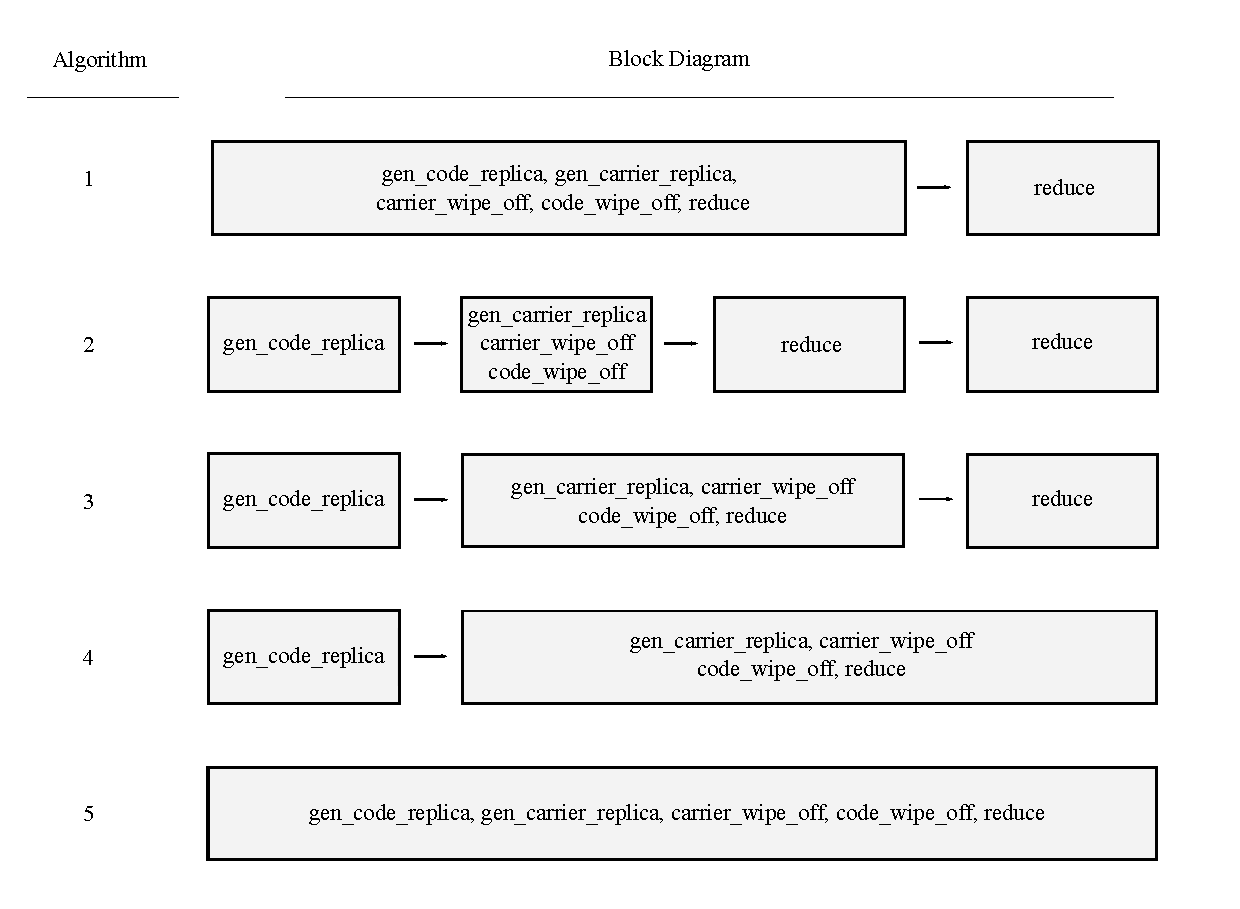
\includegraphics[width=13cm]{algorithms.pdf}}
\caption{Block-diagram description of the algorithms being tested in this paper.}
  \label{fig:algorithms}
\end{figure*}

\subsection*{Benchmarking}
Measurements of execution times are inherently noisy due to OS scheduling events, clock frequency jitter, etc. Therefore, there is a need for a statistical evaluation of the collected timings, i.e. averaging over numerous executions, performing calculations of estimators.

Runtimes in this paper were collected using the BenchmarkTools.jl package. The package tunes the execution parameters, such as the number of executions, automatically. Four estimators are provided as the benchmark result. These are the \emph{Minimum}, \emph{Median}, \emph{Mean}, and \emph{Maximum} estimators. In \cite{Chen2016} the authors of the package asses the minimum estimator, rather than median or mean, to be the most robust one, as execution times are heavily right-skewed. This renders the mean estimator heavily influenced by the outliers, and the maximum estimator being purely an outlier. Therefore the presented execution times are taken from the Minimum estimator unless otherwise noted.

\subsection*{Project Automation}
Algorithms under test and benchmarking scripts are all compounded into a Julia module utilizing the DrWatson.jl package \cite{Datseris2020}. This provides reproducibility of the results found in this paper, as the module keeps a list of all dependencies and their version and can be instantiated via a simple command. Additionally, the algorithms used for the comparison in this paper are tested utilizing the standard Julia testing ecosystem. The repository containing the source code and scripts for the benchmarks acquired and figures found in this paper can be found on Github \cite{Ozmaden2022}. Raw data obtained from the benchmarks on the platforms described in this paper is also made available \cite{Ozmaden2022_2}.

\section{Algorithm Design}\label{sec:algorithm-design}
\subsection*{CUDA}
CUDA is a programming framework published by NVIDIA for programming the GPU. Currently, it provides first-grade support for C/C++ and FORTRAN. CUDA is designed to ease the programming of parallel applications on the GPU, by providing an LLVM-based compiler for PTX, the NVIDIA GPU native Instruction Set Architecture (ISA). Albeit, effective CUDA programming requires a solid understanding of the low-level resources of the GPU. In the following, a short explanation of the CUDA framework is given. The information stems from NVIDIA'
s "CUDA C++ Programming Guide" \cite{NVIDIA2022}.

Functions executed on the GPU are referred to as \emph{kernels}. Each kernel is launched on a \emph{grid} consisting of \emph{thread-blocks}. The smallest units, \emph{threads}, are issued in a group of 32 to perform the same instruction. This grouping is called a \emph{warp}. The next level of thread grouping is called a \emph{block} or a \emph{thread-block}. These differ in their maximum allowed size depending on the hardware. CUDA provides three-dimensional indexing along the grid, and inside an individual thread-block. The product of the dimensions inside a block is fixed to the maximum number of threads per block, as expressed below
% \begin{figure}[h] 
%     \centering
%     \includegraphics[width=9cm]{cuda-grid}
%     \caption{An exemplary 2D CUDA grid consisting of 2D thread-blocks. Image from \cite{NVIDIA2022}.}
%     \label{fig:cuda-grid}
% \end{figure}
\begin{lstlisting}[language = Julia]
max_thread_per_block = threads_x * threads_y * threads_z
\end{lstlisting}
Thus, if one were to fix the $z$ and $y$ dimensions of a thread-block, the maximum allowed number of threads in the $x$ dimension can be easily found via:
\begin{lstlisting}[language = Julia]
threads_x = max_threads_per_block / threads_y * threads_z
\end{lstlisting}
On the grid level, no limits are tieing the $x, y$, and $z$ dimensions together.

Each thread executes in parallel on the GPU, meaning one of the priorities in parallelization optimization is providing the GPU with enough resources to saturate the number of threads performing calculations in parallel. This is often measured via an \emph{occupancy} metric. Kernels exhibiting high occupancy have the potential to better hide processing latencies, however, they are not per se the best performing as shown in \cite{Volkov2010}. In line with previous work on GNSS GPU signal processing, this paper strives for optimum occupancy at every kernel launch via a call to a launch configuration subroutine.

\subsection*{GPU Memory}
The knowledge of various memory resources of the GPU is essential for improving the efficiency of kernels. The memory available to all threads regardless of grouping is called the \emph{global memory} of the GPU. Inside each thread-block threads can access a \emph{shared memory}. Shared memory is faster than global memory. Additionally, each thread has its local on-chip L2 cache memory for local variables. 

Furthermore, there is another type of read-only memory available globally called \emph{texture memory} that possesses some unique properties. Firstly, the speed of accessing the texture memory is increased by caching. Secondly, spatially close memory locations addressed in an unpredictable order get a speed-up. And most importantly for the application in this paper, rules for out-of-bounds accesses and an interpolation method for non-integer indices can be defined upon allocation.

CUDA defines three texture memory addressing modes to define behavior upon an out-of-bounds access: \emph{wrap, clamp, mirror} and \emph{border}. Three interpolation methods are provided to deal with non-integer indices: \emph{linear, bilinear} and \emph{nearest neighbour} (CUDA.jl naming). Additionally, a boolean value called \emph{normalized\_coordinates} can be passed to specify if the indices are in the $[0, 1)$ range. To make use of the wrap addressing mode, the indices must be normalized. A simple example is provided in Figure \ref{fig:textmem} to illustrate the functioning of the described addressing modes.
\begin{figure}
    \centering
    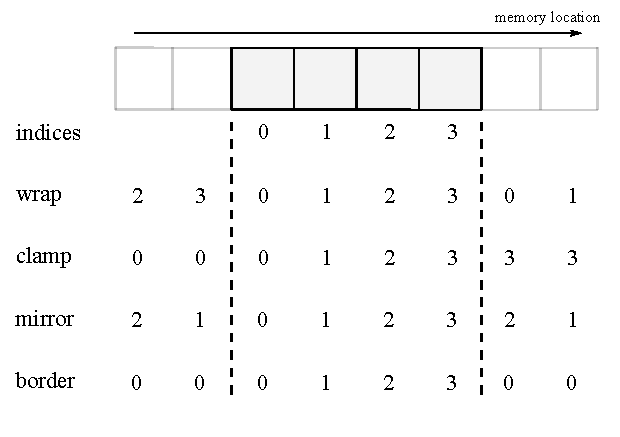
\includegraphics[scale = 0.8]{figures/texture-memory.pdf}
    \caption{\label{fig:textmem}Visualization of various addressing modes available for the texture memory in CUDA.}
\end{figure}

\subsection*{Parallel Reduction}
The cornerstone of the tracking module is the correlation process as expressed in Equation \ref{eqn:multi-correlator}. This operation requires each element of the vector to be multiplied element-wise with the others, and the result of these products must be summed over $N$ samples. While vector multiplication is trivially parallelizable, the parallelization of the sum requires some thought. Each partial sum of two elements can be computed independently of the other partial sums, however, some communication between threads is needed to facilitate a step-wise reduction of a vector of length $N$ into a scalar value. 

In his seminal work, Harris has presented ways to optimize the parallel reduction in CUDA \cite{Harris2007}. He introduces seven kernels, each subsequent improving on the preceding. The reduction strategy involves the use of a binary tree-like summing. Harris' reduction kernel numbering is taken one-to-one in the naming of the algorithms in this paper as described in Section \ref{sec:methodology}.
\begin{figure*}[t]
    \centerline{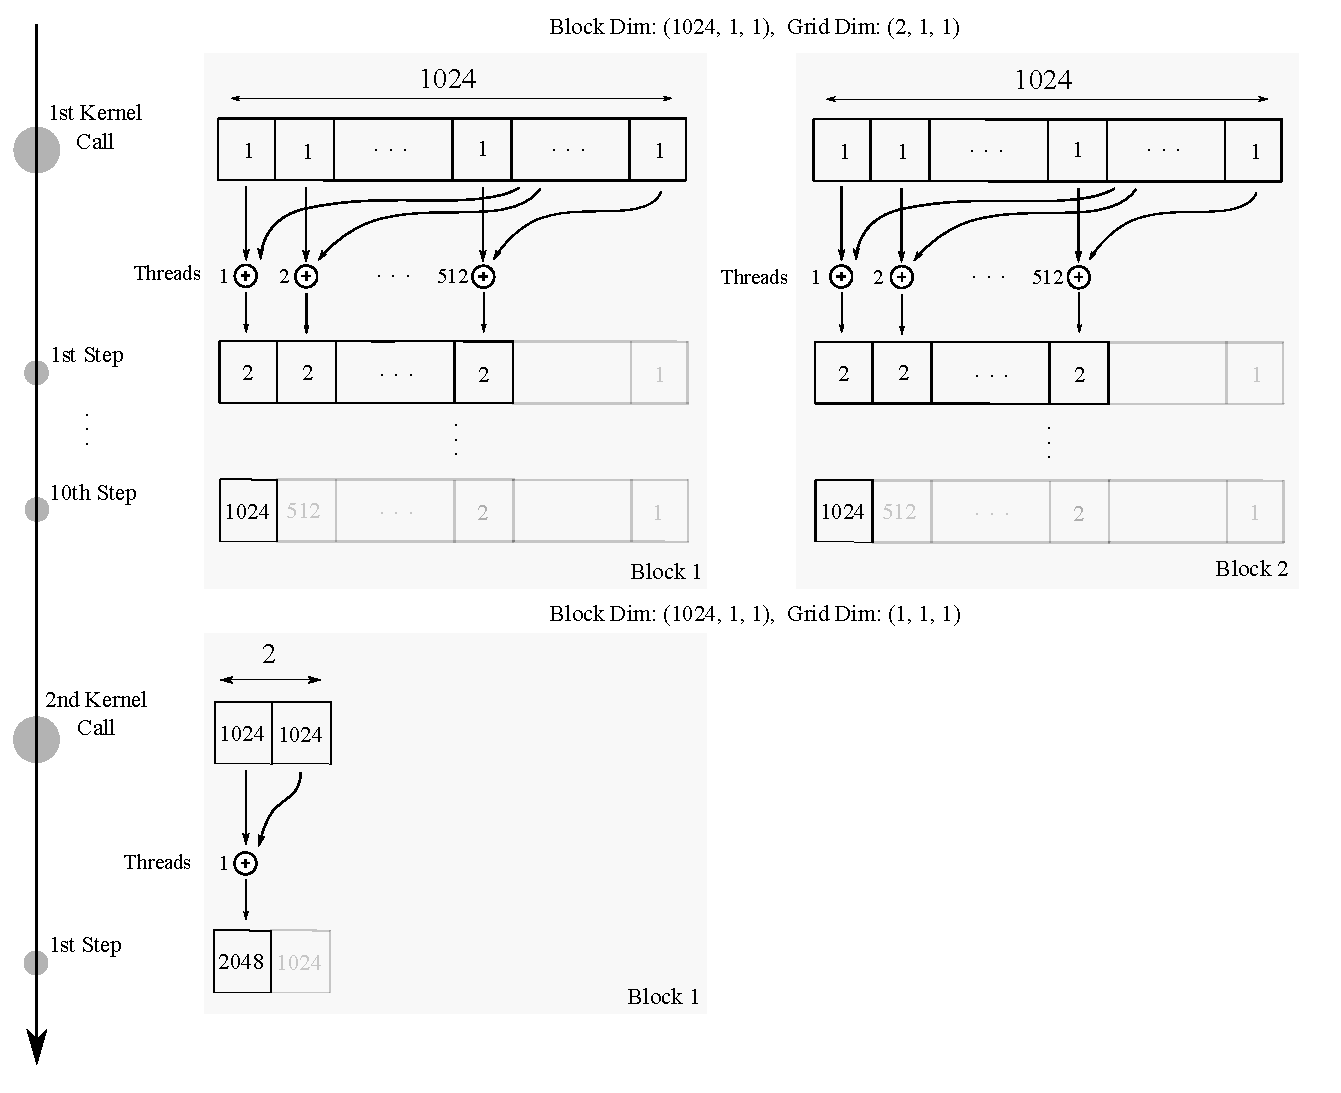
\includegraphics[width=13cm]{reduction-tree.pdf}}
    \caption{Visualization of a tree-like reduction algorithm from \cite{Harris2007}, using a coalesced memory access. The kernel is first launched on a grid of two blocks, which produce their respective partial sums for the 2nd kernel launch to sum.}
    \label{fig:reduction}
\end{figure*}

One of the main issues of parallel reduction is the innate need for synchronization between parallel threads. Before CUDA version 9, it was only possible to synchronize threads across a block. This meant that only a vector of length matching the maximum allowed threads per block could have been reduced in a \emph{single-pass} (single kernel invocation). For greater input sizes, a partial sum vector of length equal to the number of blocks has to be allocated. The second kernel invocation reduces the values of partial sums across blocks. This is called \emph{multi-pass} reduction, in contrast to \emph{single pass}. Figure \ref{fig:reduction} illustrates the multi-pass reduction over 2048 elements by using the 3rd kernel from \cite{Harris2007}.

With the introduction of \emph{Cooperative Groups} in CUDA version 9, it has become possible to synchronize GPUs at every level, including thread-blocks across a grid. Therefore, a kernel launched within a cooperative group can reduce across a block and subsequently across all blocks in a single-pass.

Another approach to summing a vector on a GPU is via the use of atomic operations. However, atomic operations come at a cost of not utilizing the full bandwidth of the GPU and therefore must be used sparingly. In this paper atomic reduction is used to eliminate the second reduction kernel call in algorithms 4 and 5 as illustrated in Figure \ref{fig:algorithms}.

\subsection*{Kernel Implementations}
There are various ways to improve the runtime efficiency of a kernel. Firstly, a distinction has to be made if the kernel is a so-called \emph{compute-bound} or a \emph{memory-bound} kernel. For compute-bound kernels, the mathematical operations performed by each thread have to be optimized. For the memory-bound ones, accesses to the memory resources are to be accelerated. 

Four operations in the tracking module have the potential to be parallelized. These are the code replica generation from Equation \ref{eqn:code-replica}, carrier replica generation from Equation \ref{eqn:carrier-replica}, downconversion, and correlation from  Equation \ref{eqn:multi-correlator}. These can be defined as separate kernels or fused in various ways as shown in Figure \ref{fig:algorithms}. The downconversion kernel is the only one of the four that can be described as a compute-bound one. The rest are memory-bound kernels and are to be optimized to reach the peak throughput of the GPU.

As discussed previously, the correlation operation involves two stages, firstly a vector element-wise multiplication, and subsequently a summation over all $N$ elements. As an example, a GPS L1 C/A signal of 1 ms duration is considered. Sampled at 2.048 MHz sampling frequency this produces 2048 I/Q samples ($N=2048
$). With an assumption of early-prompt-late correlation ($L = 3$) and four antennas ($M = 4$) this results in 48 reduction kernel invocations for each 1ms chunk. This is firstly due to the maximum amount of threads in a block, which is 1024 for both platforms from Table \ref{tab:platforms}. Therefore, a single-pass reduction with the algorithms from \cite{Harris2007} is not possible. Secondly, the reduction has to be performed on both the I and Q components of the signal.

In this paper, kernel calls are reduced by implementing extended versions of the original reduction algorithm. These are the so-called "cplx" and "cplx\_multi" kernels. The "cplx" kernel assigns each thread to deal with both in-phase and quadrature components of the signal and has to perform two passes for each $m \in M$ and $l \in L$. Whereas, the "cplx\_multi" reduction kernel is totally parallelized and performs two passes only once per $k \in K$.

The CUDA kernel currently implemented in Tracking.jl is a variant of the first algorithm from Figure \ref{fig:algorithms}, albeit without the texture memory code generation. Additionally, this is the only kernel that possesses a multi-dimensional grid. The newly devised ones in this paper are all developed to be one-dimensional kernels, assigning more workload to each thread.

% \begin{algorithm}[h]
%     \caption{\label{alg:reduce-cplx} Complex multi reduction kernel extended from Harris \#3}
    
%     \begin{algorithmic}[1]
%         \Procedure{reduce\_cplx\_multi!}{output, input}
%             \vspace{1mm}
%             \State $\mathrm{tid} \gets \mathrm{threadIdx.x}$
%             \State $\mathrm{iq\_offset} \gets \mathrm{blockDim.x}$
%             \State $\mathrm{shmem} := \mathrm{DynamicSharedMemory} \in \mathtt{F32}^{\hspace{1mm}(2N)\times M \times L}$
%             \vspace{4mm}
%             \State \# Load input into shared memory
%             \State $n = \mathrm{blockIdx.x} \times \mathrm{blockDim.x} + \mathrm{threadIdx.x}$

%             \ForAll{$m \in M,\hspace{1mm} l \in L$}
%                 \vspace{1mm}
%                 \If{$n \leq \mathrm{length(input)}$}
%                     \State $\mathrm{shmem}[\mathrm{tid} \hspace{4.8em}, m, l] \gets \mathrm{input.re}[n, m, l]$
%                     \State $\mathrm{shmem}[\mathrm{tid}+\mathrm{iq\_offset}, m, l] \gets \mathrm{input.im}[n, m, l]$
%                 \EndIf

%                 \vspace{2mm}
%                 \State $\mathrm{sync\_threads}$ 
%                 \vspace{2mm}

%                 \State \# Perform tree-like reduction in shared memory
%                 \For{$s = \mathrm{blockDim.x} \div 2,\hspace{1mm} s \neq 0 , \hspace{1mm}s = s \div 2 $}
%                     \vspace{1mm}
%                     \If{$\mathrm{tid} - 1 < s$}
%                         \State $\mathrm{shmem}[\mathrm{tid}, m, l] \gets \mathrm{shmem}[\mathrm{tid} + s, m, l]$
%                         \State $\mathrm{shmem}[\mathrm{tid}+\mathrm{iq\_offset}, m, l] \gets \mathrm{shmem}[\mathrm{tid} + s +\mathrm{iq\_offset}, m, l] $
%                         \vspace{2mm}
%                         \State $\mathrm{sync\_threads}$ 
%                     \EndIf
%                 \EndFor

%                 \vspace{4mm}
%                 \State \# First thread holds the result
%                 \If{$\mathrm{tid} == 1$}
%                     \State $\mathrm{output.re}[\mathrm{blockIdx.x}, m, l] \gets \mathrm{shmem}[1, m, l]$
%                     \State $\mathrm{output.im}[\mathrm{blockIdx.x}, m, l] \gets \mathrm{shmem}[1 + \mathrm{iq\_offset}, m, l]$
%                 \EndIf
%             \EndFor
%         \EndProcedure
%     \end{algorithmic}
% \end{algorithm}

\subsection*{Code Replica Generation from Texture Memory}
Generation of the code replica is computationally prohibitive due to the modding and flooring operations (see Equation \ref{eqn:code-replica}). The proposed receiver architecture loads all CDMA codes $c^{(k)}$ of $K$ satellites directly into the texture memory of the GPU in their original length at the beginning of the operation. At the time of writing this paper, the texture memory interface in CUDA.jl remains experimental and subject to change. An example for allocating a texture memory array is provided below. Note the specific memory adressing mode keyword argumenst passed to provide the desired functionality.
\begin{lstlisting}[language = Julia]
codes_text_mem = CuTexture(
    CuTextureArray(codes),
    address_mode = CUDA.ADDRESS_MODE_WRAP,
    interpolation = CUDA.NearestNeighbour(),
    normalized_coordinates = true
)
\end{lstlisting}
Later, a code replica can be easily generated inside a CUDA kernel as shown below:\begin{lstlisting}[language = Julia]
code_replica[thread_idx] = codes[(code_frequency/sampling_frequency * (thread_idx + latest_shift) + start_code_phase) / code_length, prn)]
\end{lstlisting}
Note that this provides the advantage of sparing the mod and floor operations, due to the selected memory addressing modes earlier.

Authors of \cite{Shi2021} have recently introduced a texture-memory-based algorithm for BeiDou signal generation by loading codes into the texture memory. However, the specific addressing and filtering modes used are not mentioned. Authors of \cite{Li2012} implement the code and carrier replica generation via tables stored in texture memory. The use of addressing modes is mentioned but the algorithm is not presented.

In this paper, the technique of code replica generation from texture memory is specifically applied to a multi-antenna GNSS receiver. Additionally, global memory and texture memory are used in cooperation, as the mutable code replica array is contained in the global memory of the GPU, initiated originally from the chip-length codes in the texture memory.

\subsection*{SIMD}
The existing codebase of Tracking.jl uses SIMD-accelerated CPU correlation. This is perfomed by utilizing the LoopVecorization.jl \footnote{https://github.com/JuliaSIMD/LoopVectorization.jl} Package. It provides user friendly macros that can be prefixed to a loop as shown below on a concrete example of the correlation operation:
\begin{lstlisting}[language = Julia]
@avx for i = start_sample:num_samples + start_sample - 1
    for j = 1:length(a_re)
        sample_shift = correlator_sample_shifts[j] - correlator_sample_shifts[1]
        a_re[j] += d_re[i] * code[i + sample_shift]
        a_im[j] += d_im[i] * code[i + sample_shift]
    end
end
\end{lstlisting}
In order to compare the effective output from programming different parallelization strategies on different hadrware in a fair manner, the GPU algorithms are benchmarked against the SIMD algorithm.

\section{Experiment Evaluation}\label{sec:analysis}

\subsection*{Reduction}
An evaluation of the "cplx\_multi" reduction introduced in Section \ref{sec:algorithm-design} is carried out. Parameters used in the experiment to assess the developed algorithm are provided in Table \ref{tab:reduction-params}. The results are provided in Figure \ref{fig:reduction-plot}. One can observe "cplx\_multi" outperforming "cplx" and "pure", due to the fusion of the kernel invocations. Therefore only "cplx\_multi" kernels are presented in this paper.

\begin{table}
  \centering
  \caption{\label{tab:reduction-params}Parameters for testing the reduction algorithms.}
  \begin{tabular}{cc}
  \multicolumn{1}{c}{Parameter Name} & \multicolumn{1}{c}{Values}  \vspace{2mm}\\ 
  Number of elements, $N$              & 2048 - 32768               \\
  Number of antennas, $M$               & 1, 4                       \\
  Number of correlators, $L$           & 3, 7                   
  \end{tabular}  
\end{table}
\begin{figure}[h]
  \centering
  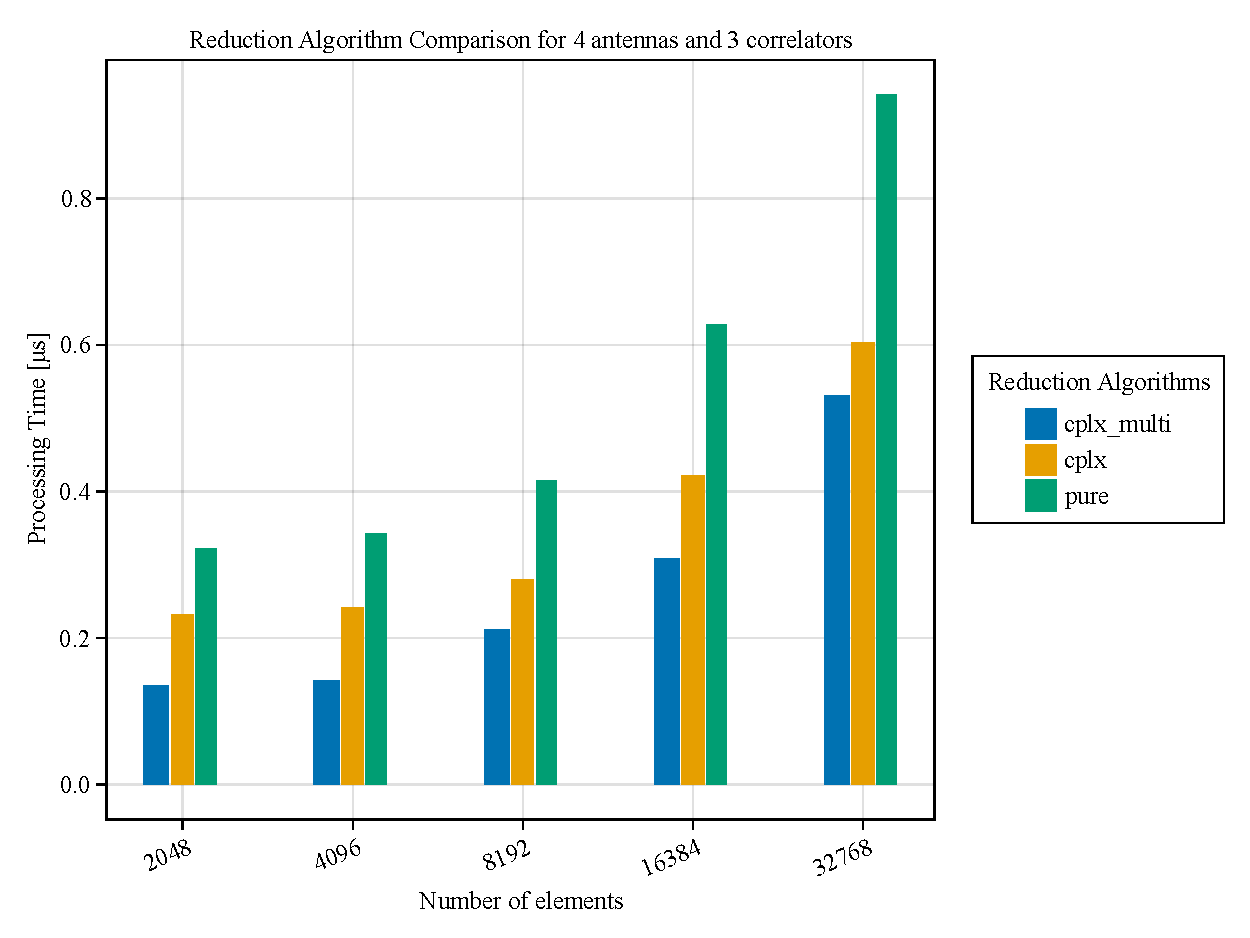
\includegraphics[scale=0.5]{reduction.pdf}
  \caption{Runtime analysis of the three reduction algorithms: "pure", "cplx", and "cplx\_multi"\label{fig:reduction-plot}}
\end{figure}


\subsection*{Texture memory}

The generation of the code replica from the texture memory of the GPU requires the use of the nearest neighbor addressing filtering and wrap addressing mode. This, however, differs in its implementation from the modding and flooring of code phases introduced in Equation \ref{eqn:code-replica}. The discrepancy results in a slightly different code phase being calculated by the algorithms generating the code replica from global memory and texture memory. An analysis of the introduced error by this algorithm is carried out. The results can be seen in Figure \ref{fig:code-phase}, along with a timing experiment against the global memory counterpart. As one can observe, the discrepancy results in a negligible relative code phase error, and the speed-up is significant. Short statistical summary is found in Table \ref{tab:code-phase-error}. It can be  concluded that the speed-up of using the code replication via texture memory is a well-founded trade-off. 

\begin{table}
  \centering
  \caption{\label{tab:code-phase-error} Statistical analysis of the relative code phase error between the global memory and texture memory code replication algorithms.}
  \begin{tabular}{rcl}
  \multicolumn{1}{l}{Minimum relative error} & \multicolumn{1}{l}{} & 0\%                       \\
  Mean relative error                        &                      & 0.03\%  \\
  Median relative error                      &                      & 0.02\%  \\
  Maximum relative error                     &                      & 3.17\% 
  \end{tabular}
\end{table}

\begin{figure*}[h]
  \centering
  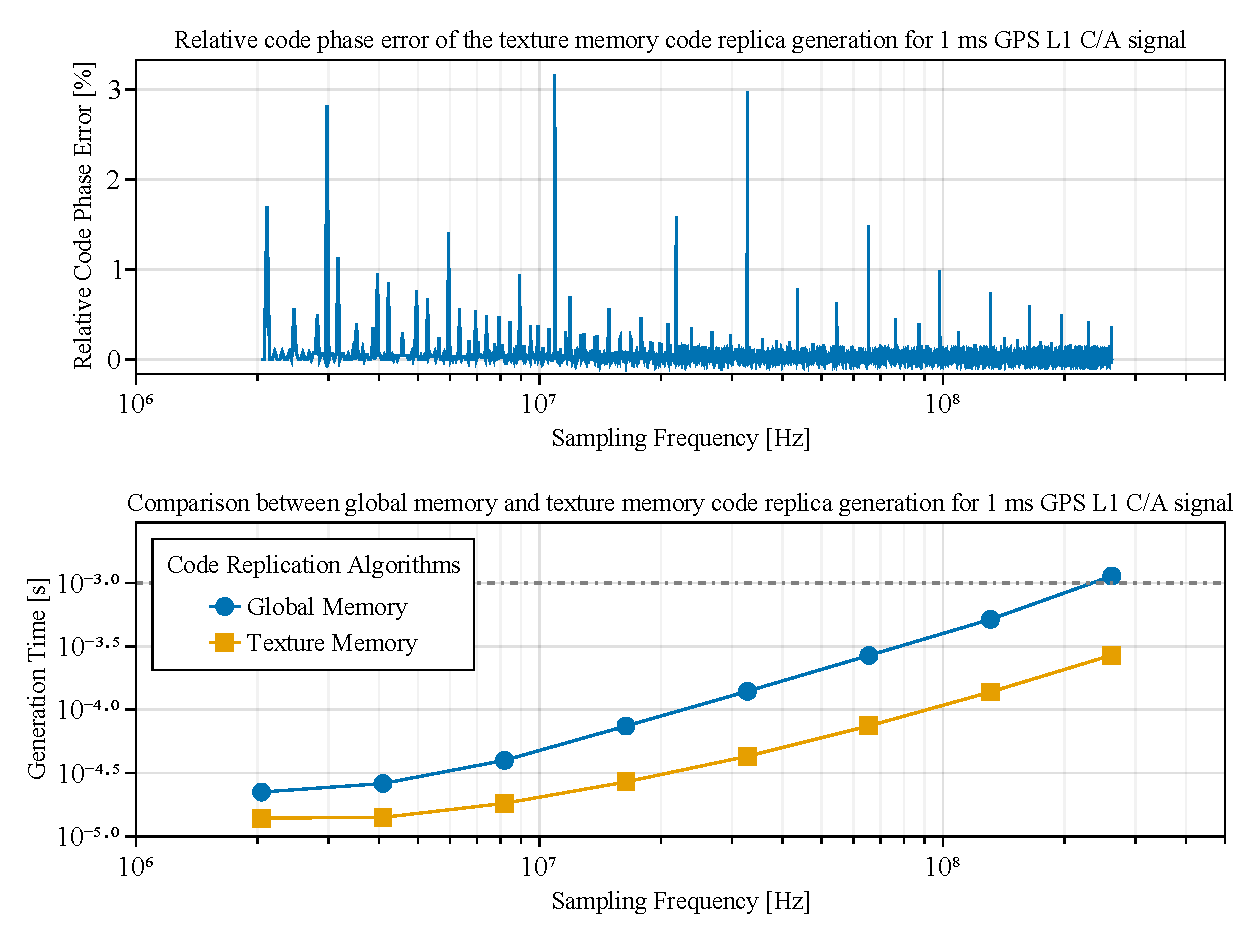
\includegraphics[width = 13cm]{code_phase.pdf}
  \caption{Above: Code phase error due to the discrepancy between global memory and texture memory code replication algorithms. Below: runtime analysis between the global and texture memory code replication algorithms. The dashed line indicates the real-time bound.\label{fig:code-phase}}
\end{figure*}

\subsection*{Algorithms}
Due to the multitude of various kernel combinations, only a few selected ones are presented in this paper. The experiment setup and related functions exist in the repository \cite{Ozmaden2022}. For the sake of brevity, only kernels with the 4th reduction algorithm are shown in this paper. They are decently performing and work effortlessly on non-power-of-two input sizes. 

Upon close analysis of Figures \ref{fig:allplots}, one can conclude the results suggest that differences between the architectures of the GPUs cannot be ignored. The algorithms performing best on Platform \#1 are the worst-performers for Platform \#2, and vice-versa. The results also suggest merit in exploring parallelization on the CPU, as the CPU SIMD algorithms from \cite{Schoenbrod2022} are found to consistently outperform the GPU on Platform \#1. This is, however, not always the case on Platform \#2. A possible explanation for this is the fact that Platform \#2 possesses an ARM chip, with SIMD capabilities unmatched to the Desktop-grade Intel Core i5-9600K. Another factor is also the higher CPU clock frequency of Platform \#1. The relative mismatch between the power of the GPU and the power of the CPU on Platform \#2, leaning towards the GPU, also plays a role. The CUDA algorithm 
currently implemented in \cite{Schoenbrod2022} is being outperformed by the algorithms devised in this paper. Overall it can be said that the 4th algorithm under the name "4\_4\_cplx\_multi\_textmem" is the best performing for most of the time on Platform \#1. Whereas algorithm 2 under the name "2\_4\_cplx\_multi\_textmem" performs the best on Platform \#2, for cases utilizing under seven correlators. This is somewhat surprising, as it suggests launch configurations of individual kernels playing a bigger role on the Jetson device, and/or that Platform \#2 has shorter API overhead. Moreover, this could be attributed to the somewhat slower atomic operations on Platform \#2, as these are utilized in algorithms 4 and 5.

The results suggest real-time operation capabilities of the developed algorithms, even under introduced multi-antenna and multi-correlator load. Most algorithms can be executed in real-time under 20 MHz sampling frequency both on Platform \#1 and \#2. Some algorithms reach around 40 MHz processing capability with 4 antennas or even 100 MHz with a single antenna and an early-prompt-late correlator. Only the case of processing GPS L5 I5 signals with 4 antennas and 7 correlators remains an unsolved challenge.


\section{Conclusion}\label{sec:conclusion}
A series of benchmarks were carried out across different GNSS tracking algorithms on the GPU and CPU. Benchmarks varied the signal input sizes through the the sampling frequency, number of antennas, and number of correlators. Simulated signals were from the GPS constellation at two frequency bands and following codes: GPS L1 C/A, GPS L5 I5. The GPU algorithms differ in their implementation of the parallel reduction, use of texture memory for code replication, and the fusion of subsequent kernels. To keep the comparison fair, GPU algorithms were benchmarked against a parallelized SIMD CPU algorithm. A comparison between the algorithms has shown differing results for the two platforms under test. For the Desktop PC, an implementation with the code replication kernel separate from a fused carrier wipe-off and single-pass reduction kernel shows the best performance for lower sampling frequencies of the receiver. The SIMD-based CPU algorithms outperform the GPU algorithms on a Desktop PC, but fall behind on the NVIDIA Jetson device. The fully separate kernel algorithm performed the best on the NVIDIA Jetson device. All developed algorithms show real-time capabilities under the assumption of 4 antennas, 3 correlators and 20 MHz sampling frequency.

\section*{Acknowledgements}
I would like to thank Tim Besard, creator and co-maintainer of CUDA.jl, for his readiness to answer questions and offer advice. The data for this paper has been gathered utilizing DrWatson.jl, and visualized by using Makie.jl \cite{Datseris2020, Danisch2021}. Parts of the research leading to this work were funded within the project ”ROSANNA” by the German Aerospace Center (DLR) on behalf of the German Federal Ministry of Economic Affairs and Energy under grant no. 50NA1901. This support is greatly acknowledged.

% **************GENERATED FILE, DO NOT EDIT**************

\bibliographystyle{juliacon}
\bibliography{ref.bib}


\newpage
% \section*{Appendix}
% \begin{figure*}[t]
%     \centerline{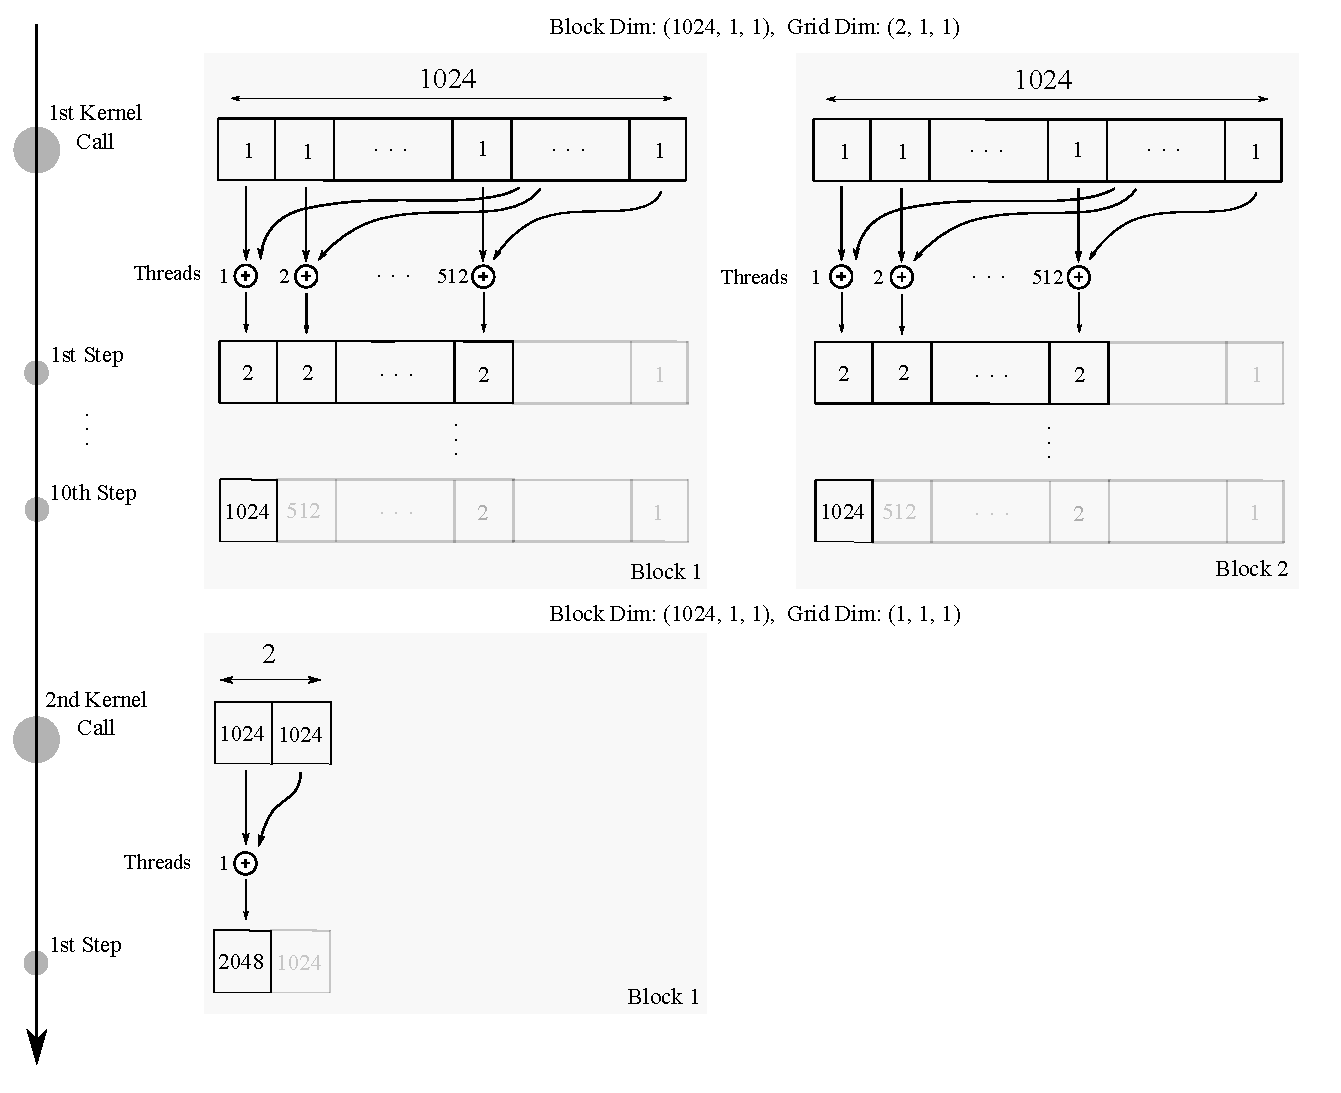
\includegraphics[width=13cm]{reduction-tree.pdf}}
%     \caption{Visualization of a tree-like reduction algorithm from \cite{Harris2007}, using a coalesced memory access. The kernel is first launched on a grid of two blocks, which produce their respective partial sums for the 2nd kernel launch to sum.}
%     \label{fig:reduction1}
% \end{figure*}

\begin{figure*}[t]
    \centerline{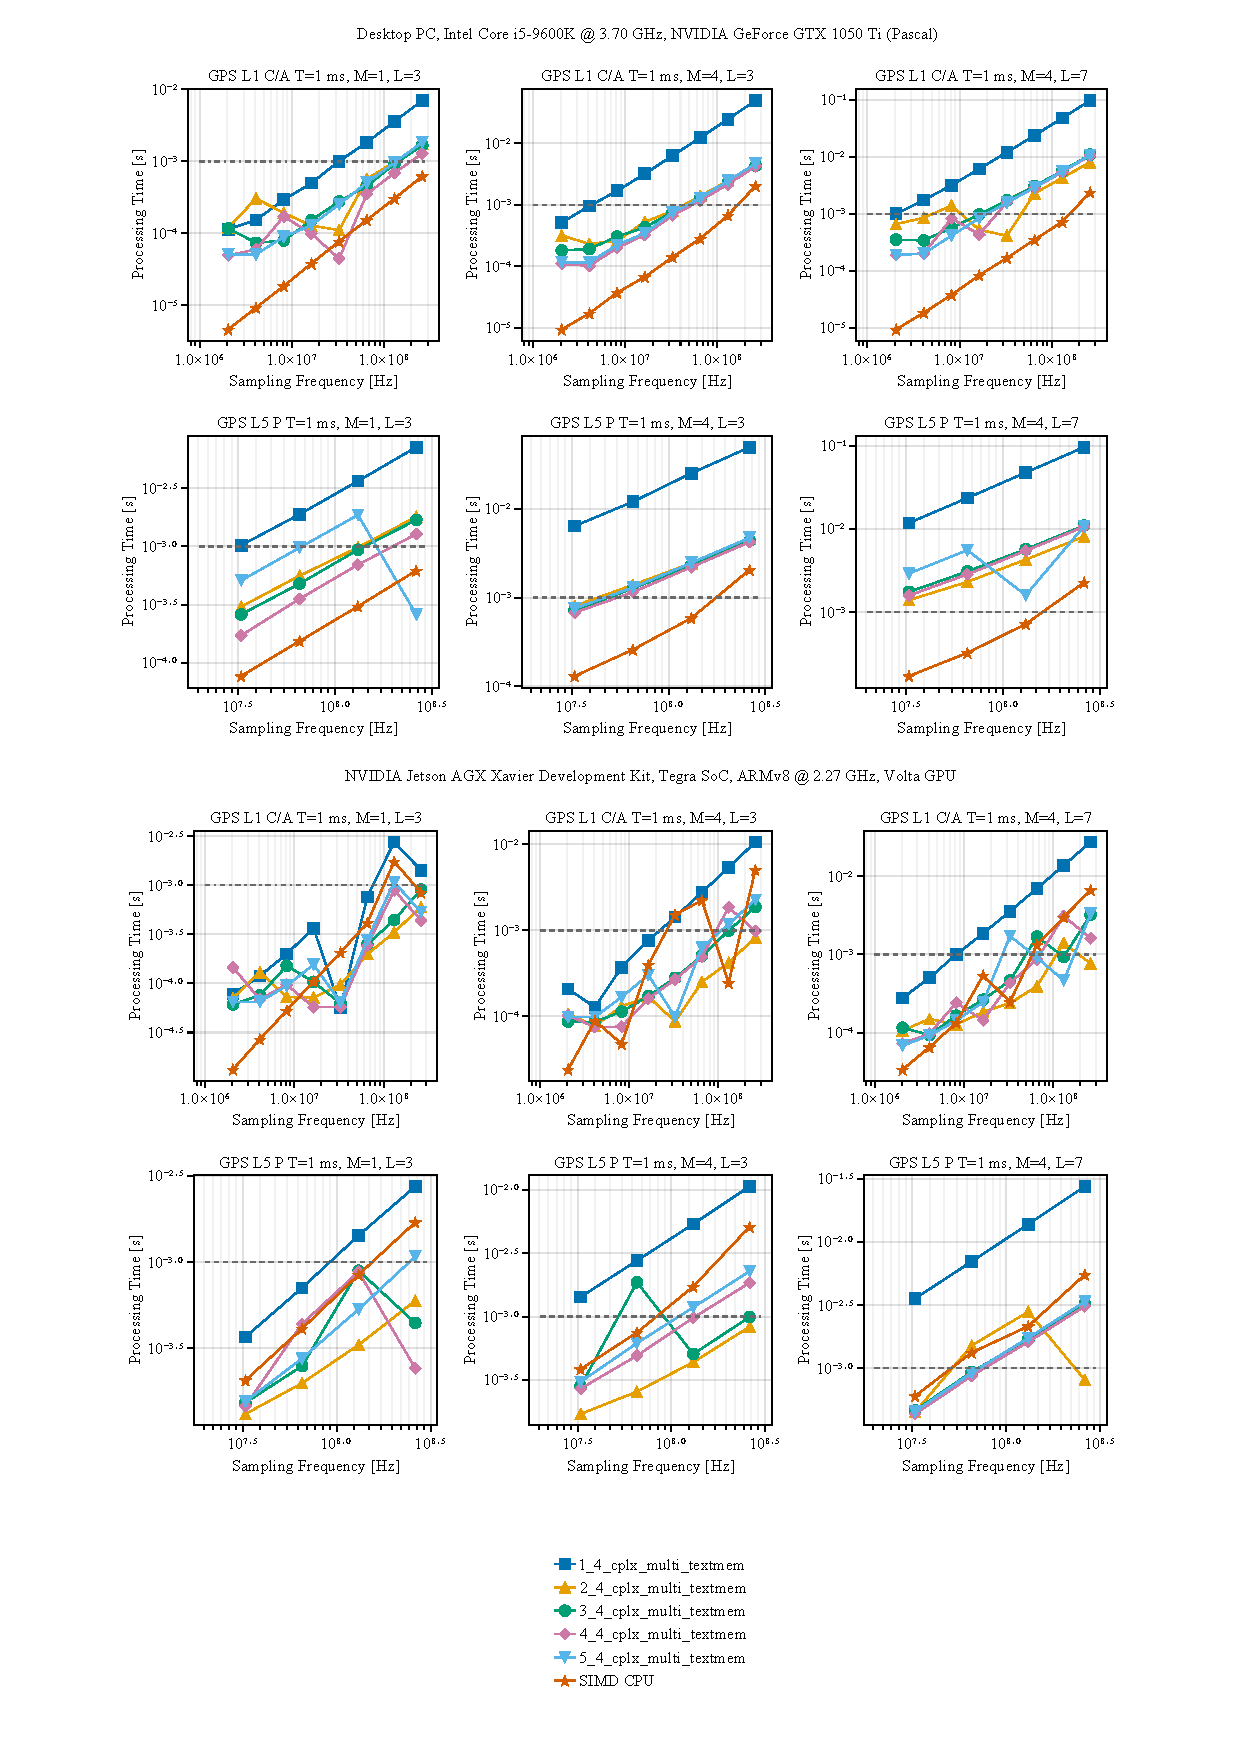
\includegraphics[scale = .8]{allplots.pdf}}
    \caption{Above: Processing time of correlation of a 1ms GPS signal on Platform \#1. Below: Processing time of correlation of a 1ms GPS signal on Platform \#2. The dashed line indicates the real-time processing bound.\label{fig:allplots}}
 \end{figure*}
 
\end{document}

% Inspired by the International Journal of Computer Applications template
